\chapter{Empirical Analysis}

\fbox{
    \parbox{\textwidth}
    {
        Chapter Overview
        \begin{itemize}
            \item Applying Bayesian \acp{cnn} for the task of Image Recognition on MNIST, CIFAR-10, CIFAR-100 and STL-10 datasets.
            \item Comparison of results of Bayesian \acp{CNN} with Normal \acp{cnn} architectures on similar datasets.
            \item Regularization effect of Bayesian Network with dropouts.
            \item Distribution of mean and variance in Bayesian \acp{cnn} over time. 
            \item Parameters comparison before and after model pruning. 
        \end{itemize}
    }
}

\pagebreak

\section{Experimentation Methodology} \label{experiments}

\subsubsection{Activation Function}

The originally chosen activation functions in all architectures are \textit{ReLU}, but we must introduce another, called \textit{Softplus}, see \eqref{softplus}, because of our method to apply two convolutional or fully-connected operations. As aforementioned, one of these is determining the mean $\mu$, and the other the variance $\alpha \mu^2$. Specifically, we apply the \textit{Softplus} function because we want to ensure that the variance $\alpha \mu^2$ never becomes zero. This would be equivalent to merely calculating the MAP, which can be interpreted as equivalent to a maximum likelihood estimation (MLE), which is further equivalent to utilising single point-estimates, hence frequentist inference. The \textit{Softplus} activation function is a smooth approximation of \textit{ReLU}. Although it is practically not influential, it has the subtle and analytically important advantage that it never becomes zero for $x \rightarrow -\infty$, whereas \textit{ReLU} becomes zero for $x \rightarrow -\infty$.
\\ 
\begin{equation}\label{softplus}
     \text{Softplus}(x) = \frac{1}{\beta} \cdot \log \big ( 1 + \exp(\beta \cdot x) \big )
\end{equation}
\\
where $\beta$ is by default set to $1$.
\newline All experiments are performed with the same hyper-parameters settings as stated in the Appendix.

\subsubsection{Network Architecture}

For all conducted experiments, we implement the foregoing description of Bayesian \acp{cnn} with variational inference in LeNet-5 \cite{lecun1998gradient} and AlexNet \cite{krizhevsky2012imagenet}. The exact architecture specifications can be found in the Appendix and in our GitHub repository\footnote{\url{https://github.com/kumar-shridhar/PyTorch-BayesianCNN}}.

\subsubsection{Objective Function}
TO learn the objective function, we use \textit{Bayes by Backprop} \cite{graves2011practical, blundell2015weight}, which is a variational inference method to learn the posterior distribution on the weights $w \sim q_{\theta}(w|\mathcal{D})$ of a neural network from which weights $w$ can be sampled in backpropagation. 
It regularises the weights by minimising a compression cost, known as the variational free energy or the expected lower bound on the marginal likelihood.

Since the true posterior is typically intractable, an approximate distribution $q_{\theta}(w|\mathcal{D})$ is defined that is aimed to be as similar as possible to the true posterior $p(w|\mathcal{D})$, measured by the Kullback-Leibler (KL) divergence \cite{kullback1951information}. Hence, we define the optimal parameters $\theta^{opt}$ as
\begin{equation}
    \begin{aligned} \label{KL}
        \theta^{opt}&=\underset{\theta}{\text{arg min}}\ \text{KL} \ [q_{\theta}(w|\mathcal{D})\|p(w|\mathcal{D})] \\
        &=\underset{\theta}{\text{arg min}}\ \text{KL} \ [q_{\theta}(w|\mathcal{D})\|p(w)] \\ & -\mathbb{E}_{q(w|\theta)}[\log p(\mathcal{D}|w)]+\log p(\mathcal{D})
    \end{aligned}
\end{equation}

where
\begin{equation}
    \text{KL} \ [q_{\theta}(w|\mathcal{D})\|p(w)]= \int q_{\theta}(w|\mathcal{D})\log\frac{q_{\theta}(w|\mathcal{D})}{p(w)}dw .
\end{equation}
This derivation forms an optimisation problem with a resulting cost function widely known as \textit{variational free energy} \cite{neal1998view,yedidia2005constructing,friston2007variational} which is built upon two terms: the former, $\text{KL} \ [q_{\theta}(w|\mathcal{D})\|p(w)]$, is dependent on the definition of the prior $p(w)$, thus called complexity cost, whereas the latter, $\mathbb{E}_{q(w|\theta)}[\log p(\mathcal{D}|w)]$, is dependent on the data $p(\mathcal{D}|w)$, thus called likelihood cost. 
The term $\log p(\mathcal{D})$ can be omitted in the optimisation because it is constant.
\newline Since the KL-divergence is also intractable to compute exactly, we follow a stochastic variational method \cite{graves2011practical,blundell2015weight}.
We sample the weights $w$ from the variational distribution $q_{\theta}(w|\mathcal{D})$ since it is much more probable to draw samples which are appropriate for numerical methods from the variational posterior $q_{\theta}(w|\mathcal{D})$ than from the true posterior $p(w|\mathcal{D})$. Consequently, we arrive at the tractable cost function \eqref{cost} which is aimed to be optimized, i.e. minimised w.r.t. $\theta$, during training:
\begin{equation} \label{cost}
    \mathcal{F}(\mathcal{D}, \theta)\approx \sum_{i=1}^n \log q_{\theta}(w^{(i)}|\mathcal{D})-\log p(w^{(i)})-\log p(\mathcal{D}|w^{(i)})
\end{equation}
%
where $n$ is the number of draws.

Let's break the Objective Function in \eqref{cost} and discuss in more details. 
\subsubsection{Variational Posterior }

The first term in the equation \eqref{cost} is the variational posterior. The variational posterior is taken as Gaussian distribution centered around mean $\mu$ and variance as $\sigma^2$. 

\begin{equation}
    q_{\theta}(w^{(i)}|\mathcal{D})= \prod_{i} \mathcal{N}(w_{i} | \mu,\sigma^2)
\end{equation}

We will take the log and the log posterior is defined as :

\begin{equation}
    log(q_{\theta}(w^{(i)}|\mathcal{D}))= \sum_{i}log \mathcal{N}(w_{i} | \mu,\sigma^2)
\end{equation}

\subsubsection{Prior}

The second term in the equation \eqref{cost} is the prior over the weights and we define the prior over the weights as a product of individual Gaussians :

\begin{equation}
    p(w^{(i)})= \prod_{i} \mathcal{N}(w_{i} | 0,\sigma_{p}^2)
\end{equation}

We will take the log and the log prior is defined as:

\begin{equation}
    log (p(w^{(i)}))= \sum_{i} log \mathcal{N}(w_{i} | 0,\sigma_{p}^2)
\end{equation}

\subsubsection{ Likelihood }

The final term of the equation \eqref{cost} $\log p(\mathcal{D}|w^{(i)})$ is the likelihood term and is computed using the softmax function.

\subsubsection{Parameter Initialization}

We use a Gaussian distribution and we store mean and variance values instead of just one weight. The way mean $\mu$ and variance $\sigma$ is computed is defined in the previous chapter. Variance cannot be negative and it is ensured by using \textit{softplus} as activation function. We express variance $\sigma$ as $\sigma_{i}=softplus(\rho_{i})$ where $\rho$ is an unconstrained parameter. \\

We take the Gaussian distribution and initialize mean $\mu$ as 0 and variance $\sigma$ (and hence $\rho$) as very small number. We perform gradient descent over $\theta$ = ($\mu$, $\rho$), and individual weight $w_{i} \sim \mathcal{N} (w_{i} | \mu_{i}, \sigma_{i}$).  

\subsubsection{Optimizer}

For all our tasks, we take Adam optimizer \cite{KingmaB14} to optmize the parameters. We also perform the local reparameterization trick as mentioned in the previous section and take the gradient of the combined loss function with respect to the variational parameters ($\mu$, $\rho$).

\subsubsection{Model Pruning}

We take the weights of all the layers of the network, apply a L1 norm over it and for all the weights value as 0 are removed and the model is pruned. \\ Also, since the Bayesian \acp{cnn} has twice the number of parameters ($\mu$, $\sigma$) compared to a frequentist network (only 1 weight), we reduce the size of our network to half (AlexNet and LeNet- 5) by reducing the number of filters to half. The architecure used is mentioned in the last section of this chapter.

\section{Case Study 1: Small Datasets (MNIST, CIFAR-10)}

We train the networks with the MNIST dataset of handwritten digits \cite{lecun1998gradient}, and CIFAR-10 dataset \cite{krizhevsky2009learning} since these datasets serve widely as benchmarks for \acp{cnn}' performances. 

\subsection{Datasets}
\newline
\subsubsection{MNIST}
The MNIST database \cite{lecun-mnisthandwrittendigit-2010} of handwritten digits, has a training set of 60,000 examples, and a test set of 10,000 examples. It is a subset of a larger set available from NIST. The digits have been size-normalized and centered in a fixed-size image of 28 by 28 pixels. Each image is grayscaled and is labelled with its corresponding class that ranges from zero to nine.
\newline

\subsubsection{CIFAR-10}
The CIFAR-10 are labeled subsets of the 80 million tiny images dataset \cite{Torralba:2008:MTI:1444381.1444403}. The CIFAR-10 dataset has a training dataset of 50,000 colour images in 10 classes, with 5,000 training images per class, each image 32 by 32 pixels large. There are 10000 images for testing. 
\newline

\subsection{Results}
First, we evaluate the performance of our proposed method, Bayesian \acp{cnn} with variational inference. Table \ref{tab:results} shows a comparison of validation accuracies (in percentage) for architectures trained by two disparate Bayesian approaches, namely variational inference, i.e. \textit{Bayes by Backprop} and Dropout as proposed by Gal and Ghahramani \cite{gal2015bayesian}.\\

We compare the results of these two approaches to frequentist inference approach for both the datasets. Bayesian \acp{cnn} trained by variational inference achieve validation accuracies comparable to their counter-architectures trained by frequentist inference. On MNIST, validation accuracies of the two disparate Bayesian approaches are comparable, but a Bayesian LeNet-5 with Dropout achieves a considerable higher validation accuracy on CIFAR-10, although we were not able to reproduce these reported results.
\begin{table}[H]
\tiny
    \centering
    \renewcommand{\arraystretch}{1.5}
    \resizebox{\linewidth}{!}{
    \begin{tabular}{ l  c  c  c  c } 
     \hline
      \empty & MNIST & CIFAR-10   \\ [0.75ex]
     \hline
     Bayesian AlexNet (with VI) & 99 & 73   \\
     
     Frequentist AlexNet & 99 & 73   \\
     \hdashline
     Bayesian LeNet-5 (with VI) & 98 & 69   \\
     
     Frequentist LeNet-5 & 98 & 68   \\
     \hdashline
     Bayesian LeNet-5 (with Dropout) & 99.5 & 83  \\ 
     \hline \\
    \end{tabular}}
    \renewcommand{\arraystretch}{1.5}
    \caption{Comparison of validation accuracies (in percentage) for different architectures with variational inference (VI), frequentist inference and Dropout as a Bayesian approximation as proposed by Gal and Ghahramani \cite{gal2015bayesian} for MNIST, and CIFAR-10.}
    \label{tab:results}
\end{table}

\begin{figure}[t!] 
\begin{center}
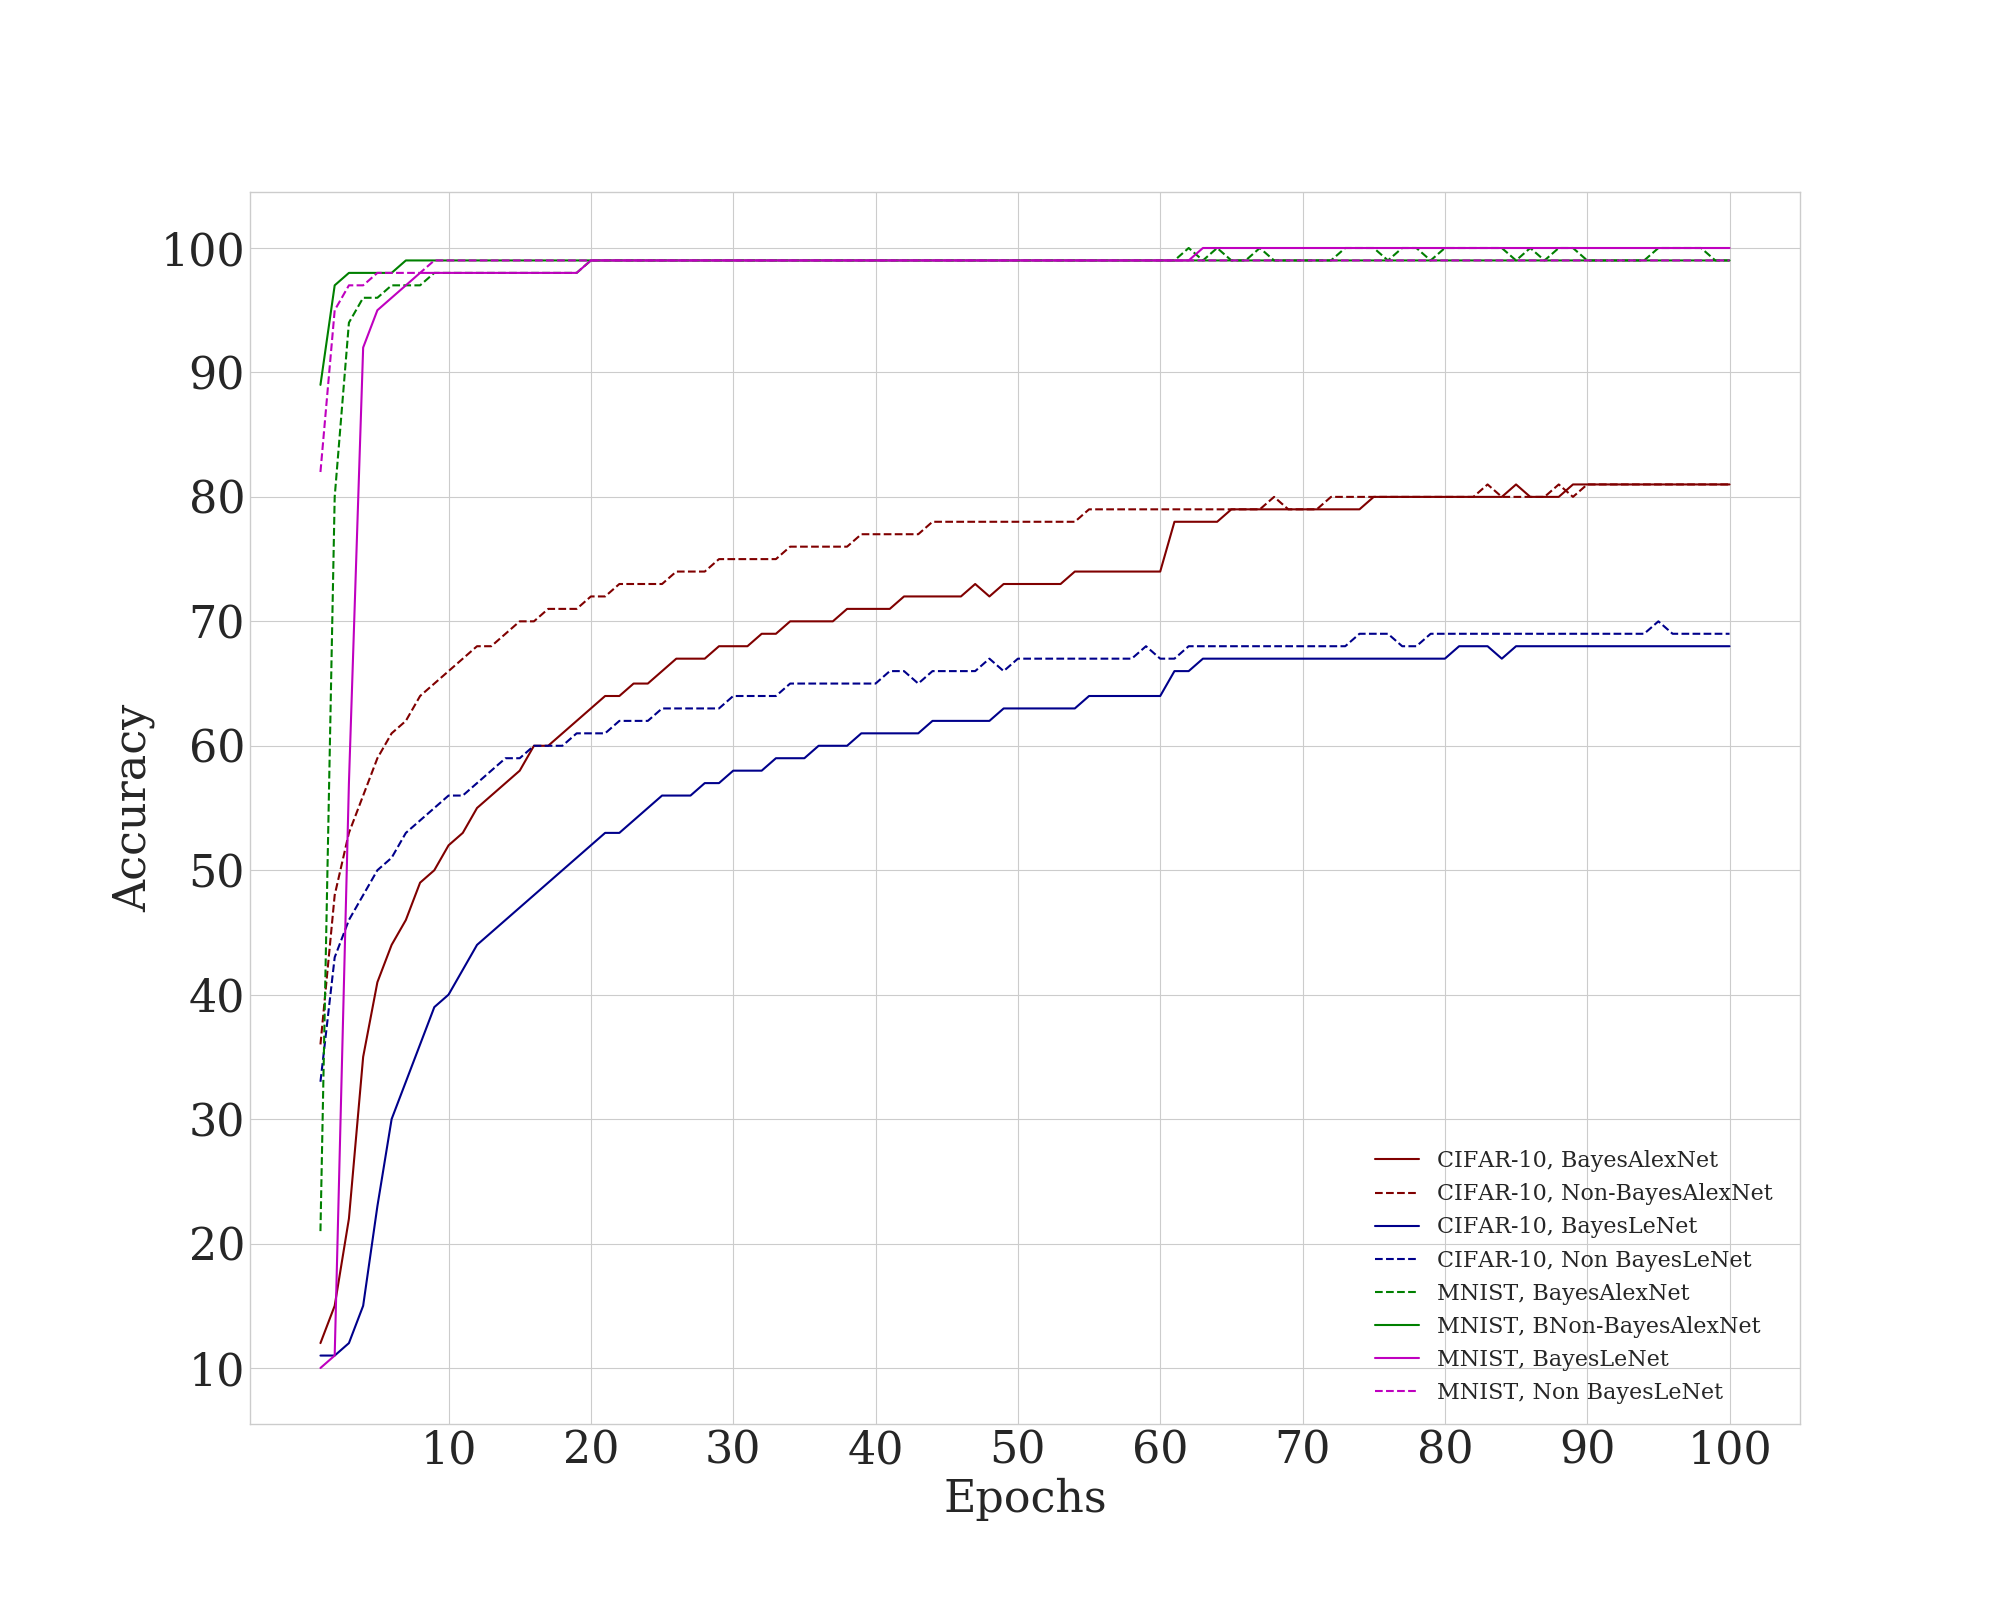
\includegraphics[width=\linewidth]{Chapter5/Figs/results_mnist_CIFAR10.png}
\caption{Comparison of Validation Accuracies of Bayesian AlexNet and LeNet-5 with frequentist approach on MNIST and CIFAR-10 datasets}
\label{fig:MnistCIFAR10reesults}
\end{center}
\end{figure} 

\newline Figure \ref{fig:MnistCIFAR10reesults} shows the validation accuracies of Bayesian vs Non-Bayesian \acp{cnn}. One thing to observe is that in initial epochs, Bayesian \acp{cnn} trained by variational inference start with a low validation accuracy compared to architectures trained by frequentist inference. This must deduce from the initialization of the variational posterior probability distributions $q_{\theta}(w|\mathcal{D})$ as uniform distributions, while initial point-estimates in architectures trained by frequentist inference are randomly drawn from a standard Gaussian distribution. (For uniformity, we changed the initialization of frequentist architecures from Xavier initialization to standard Gaussian). The latter initialization method ensures the initialized weights are neither too small nor too large. In other words, the motivation of the latter initialization is to start with weights such that the activation functions do not let them begin in saturated or dead regions. This is not true in case of uniform distributions and hence, Bayesian \acp{cnn}' starting validation accuracies can be comparably low.

\pagebreak
\newline Figure \ref{fig:std_CNN} displays the convergence of the standard deviation $\sigma$ of the variational posterior probability distribution $q_{\theta}(w|\mathcal{D})$ of a random model parameter over epochs. As aforementioned, all prior probability distributions $p(w)$ are initialized as uniform distributions. The variational posterior probability distributions $q_{\theta}(w|\mathcal{D})$ are approximated as Gaussian distributions which become more confident as more data is processed - observable by the decreasing standard deviation over epochs in Figure \ref{fig:std_CNN}. Although the validation accuracy for MNIST on Bayesian LeNet-5 has already reached 99\%, we can still see a fairly steep decrease in the parameter's standard deviation. In Figure \ref{fig:distribution}, we plot the actual Gaussian variational posterior probability distributions $q_{\theta}(w|\mathcal{D})$ of a random parameter of LeNet-5 trained on CIFAR-10 at some epochs.
%
\begin{figure}[H] 
\begin{center}
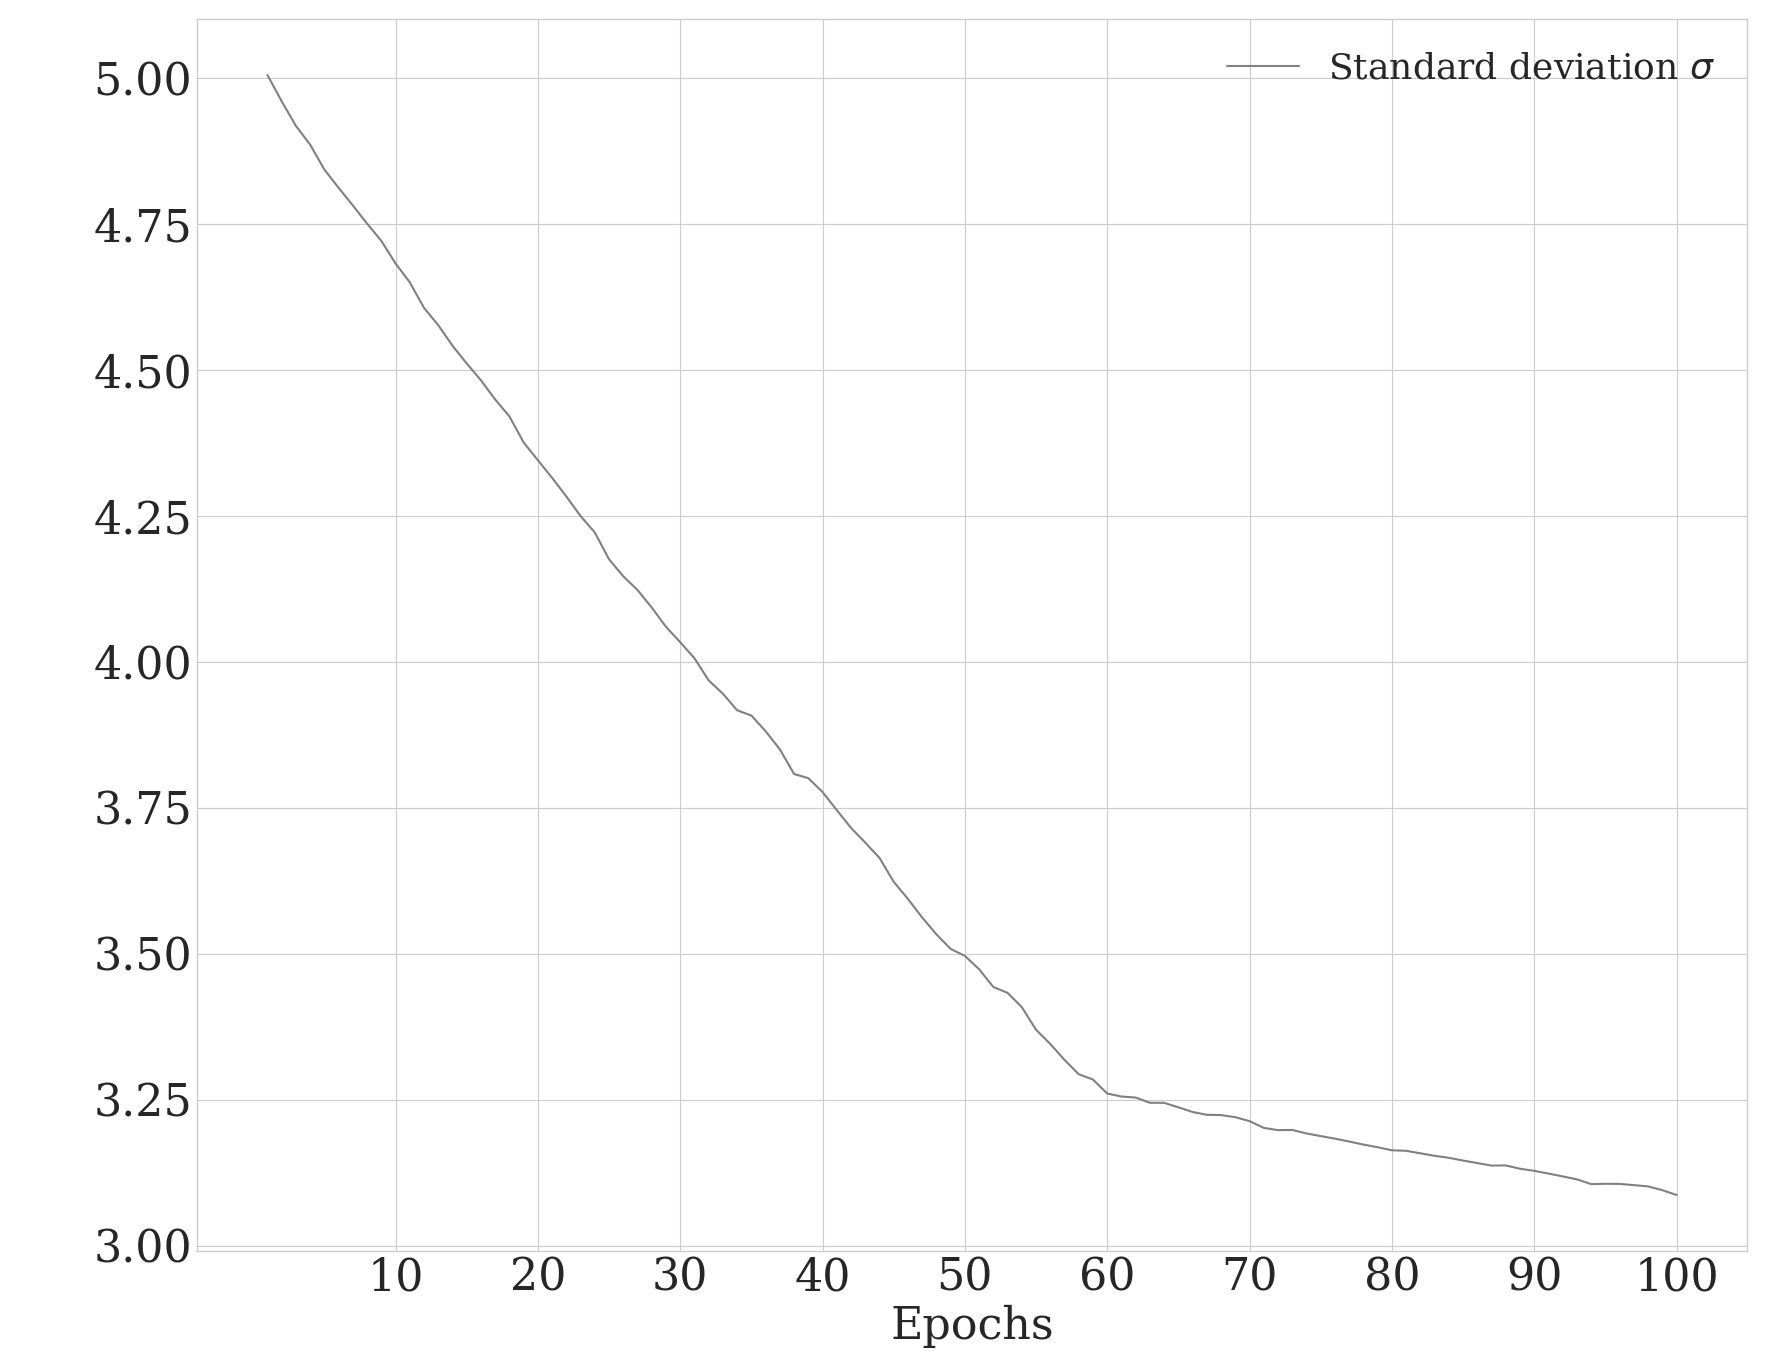
\includegraphics[width=\linewidth]{Chapter5/Figs/std_CNN.png}
\caption{Convergence of the standard deviation of the Gaussian variational posterior probability distribution $q_{\theta}(w|\mathcal{D})$ of a random model parameter at epochs 1, 5, 20, 50, and 100. MNIST is trained on Bayesian LeNet-5.}
\label{fig:std_CNN}
\end{center}
\end{figure} 
%

\begin{figure}[H] 
\begin{center}
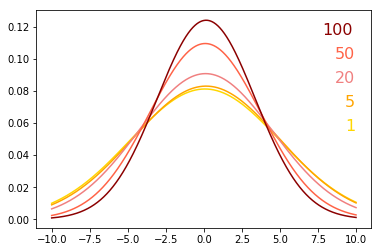
\includegraphics[width=\linewidth]{Chapter5/Figs/distribution.png}
\caption{Convergence of the Gaussian variational posterior probability distribution $q_{\theta}(w|\mathcal{D})$ of a random model parameter at epochs 1, 5, 20, 50, and 100. CIFAR-10 is trained on Bayesian LeNet-5.}
\label{fig:distribution}
\end{center}
\end{figure} 

\newline Figure \ref{fig:distribution} displays the convergence of the Gaussian variational probability distribution of a weight taken randomly from the first layer of LeNet-5 architecuture. The architecture is trained on CIFAR-10 with a 



\section{Case Study 2: Large Dataset (CIFAR-100)}
\subsection{Dataset}

\subsubsection{CIFAR-100}
This dataset is similar to the CIFAR-10, and is a labeled subset of the 80 million tiny images dataset \cite{Torralba:2008:MTI:1444381.1444403}. The dataset has 100 classes containing 600 images each. There are 500 training images and 100 validation images per class. The images are colored with a resolution of 32 by 32 pixels.

\subsection{Results}

\begin{table}[H]
\tiny
    \centering
    \renewcommand{\arraystretch}{1.5}
    \resizebox{\linewidth}{!}{
    \begin{tabular}{ l  c  c  } 
     \hline
      \empty & CIFAR-100  \\ [0.75ex]
     \hline
     Bayesian AlexNet (with VI)  & 36  \\
     
     Frequentist AlexNet & 38  \\

     Bayesian LeNet-5 (with VI) &  31  \\
     
     Frequentist LeNet-5  & 33  \\
     \hline \\
    \end{tabular}}
    \renewcommand{\arraystretch}{1.5}
    \caption{Comparison of validation accuracies (in percentage) for different architectures with variational inference (VI), frequentist inference and Dropout as a Bayesian approximation as proposed by Gal and Ghahramani \cite{gal2015bayesian} for MNIST, CIFAR-10, and CIFAR-100.}
    \label{tab:resultsCIFAR-100}
\end{table}



In Figure \ref{fig:regularization}, we show how Bayesian networks incorporate naturally effects of regularization, exemplified on AlexNet. While an AlexNet trained by frequentist inference without any regularization overfits greatly on CIFAR-100, an AlexNet trained by Bayesian inference on CIFAR-100 does not. It performs equivalently to an AlexNet trained by frequentist inference with three layers of Dropout after the first, fourth, and sixth layers in the architecture.

\begin{figure}[H] 
\begin{center}
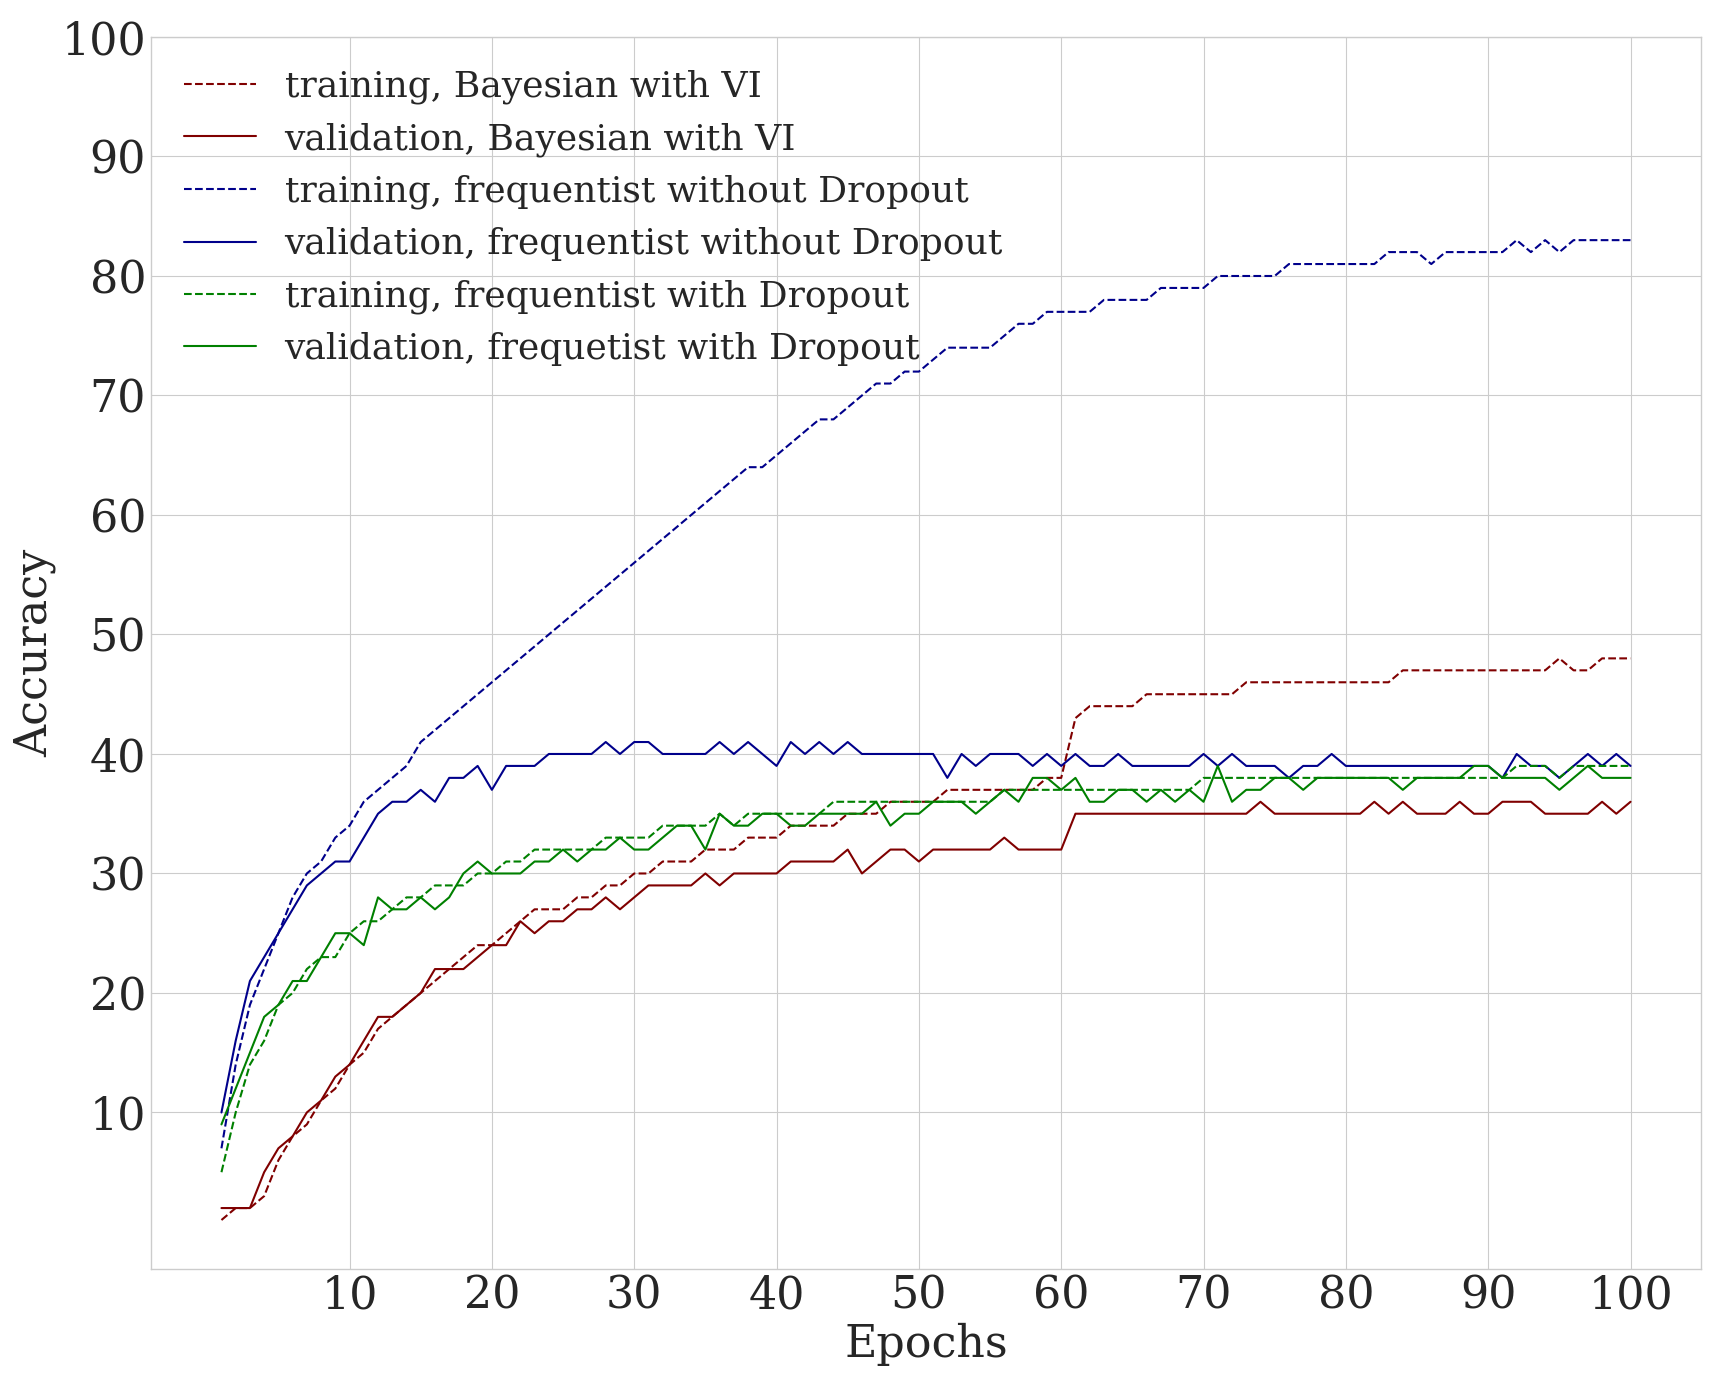
\includegraphics[width=\linewidth]{Chapter5/Figs/results_regularization.png}
\caption{Comparison of Training and Validation Accuracies of Bayesian AlexNet and LeNet-5 with frequentist approach with and without dropouts on CIFAR-100 datasets}
\label{fig:regularization}
\end{center}
\end{figure} 

\section{Uncertainity estimation}

\newline Finally, Table \ref{tab:uncertainty} compares the means of aleatoric and epistemic uncertainties for a Bayesian LeNet-5 with variational inference on MNIST and CIFAR-10. The aleatoric uncertainty of CIFAR-10 is about twenty times as large as that of MNIST. Considering that the aleatoric uncertainty measures the irreducible variability and depends on the predicted values, a larger aleatoric uncertainty for CIFAR-10 can be directly deduced from its lower validation accuracy and may be further due to the smaller number of training examples. The epistemic uncertainty of CIFAR-10 is about fifteen times larger than that of MNIST, which we anticipated, since epistemic uncertainty decreases proportional to validation accuracy. 
\begin{table}[t!]
\tiny
    \centering
    \renewcommand{\arraystretch}{1.5}
    \resizebox{\linewidth}{!}{
    \begin{tabular}{ l  c  c  c  } 
     \hline
      \empty & Aleatoric uncertainty &  Epistemic uncertainty  \\ [0.75ex]
     \hline
     Bayesian LeNet-5 (MNIST) & 0.0096 & 0.0026   \\
     
     Bayesian LeNet-5 (CIFAR-10) & 0.1920 & 0.0404   \\
     \hline \\
    \end{tabular}} 
    \renewcommand{\arraystretch}{1.5}
    \caption{Aleatoric and epistemic uncertainty for Bayesian LeNet-5 calculated for MNIST and CIFAR-10, computed as proposed by Kwon et al. \cite{kwon2018uncertainty}.}
    \label{tab:uncertainty}
\end{table}

\section{Model Pruning}

\subsubsection{Halving the Parameters number}

For every parameter for a frequentist inference network, Bayesian \acp{cnn} has two parameters ($\mu$, $\sigma$). Halving the number of parameters of Bayesian AlexNet ensures the number of parameters of it are comparable with a frequentist inference network. The number of filtres of ALexNet are halved and a new architecture called AlexNetHalf is defined in Figure \ref{tab:AlexNetHalfArchitecture}. 

\begin{table}[h!]
    \centering
    \renewcommand{\arraystretch}{2}
    \begin{tabular}{c c c c c c} 
 \hline
 layer type & width & stride & padding & input shape & nonlinearity \\ [0.5ex] 
 \hline
 convolution ($11\times11$) & 32 & 4 & 5 & $M\times3\times32\times32$ & Softplus \\ 
 
 max-pooling ($2\times2$) & \empty & 2 & 0 & $M\times32\times32\times32$ & \empty \\
 
 convolution ($5\times5$) & 96 & 1 & 2 & $M\times32\times15\times15$ & Softplus \\
 
 max-pooling ($2\times2$) & \empty & 2 & 0 & $M\times96\times15\times15$ & \empty \\
 
 convolution ($3\times3$) & 192 & 1 & 1 & $M\times96\times7\times7$ & Softplus \\
 
 convolution ($3\times3$) & 128 & 1 & 1 & $M\times192\times7\times7$ & Softplus \\
 
 convolution ($3\times3$) & 64 & 1 & 1 & $M\times128\times7\times7$ & Softplus \\
 
 max-pooling ($2\times2$) & \empty & 2 & 0 & $M\times64\times7\times7$ & \empty \\
 
 fully-connected & 64 & \empty & \empty & $M\times64$ & \empty \\ [1ex] 
 \hline
\end{tabular}
\renewcommand{\arraystretch}{1.5}
\label{tab:AlexNetHalfArchitecture}
\caption{AlexNetHalf with number of filters halved compared to the original architecture.}
\end{table}


The AlexNetHalf architecture was trained and validated on the MNIST and CIFAR10 dataset and the results are shown in Table \ref{tab:resultsAlexNetHalf}. The accuracy of pruned AlexNet with only half the number of filters compared to the normal architecture shows an accuracy gain of 6 percent in case of CIFAR10 and equivalent performance for MNIST dataset. Lesser filters learn the most important features which proved better at inter-class classification is one of the explaination for it. Upon visualization of the filters, no distinct clearification can be made to prove the previous statement.  
Another possible explaination could be the model is fitting perfectly after reducing the number of filters ensuring the model is not overfitting and validation accuracy is comparitively higher. CIFAR-100 higher validation accuracy on ALexNetHalf and a lower training accuracy than Bayesian AlexNet proves the theory. Using lesser number of filters further enhances the regularization effect and makes the model more robust against overfitting. 

\begin{table}[H]
\tiny
    \centering
    \renewcommand{\arraystretch}{1.5}
    \resizebox{\linewidth}{!}{
    \begin{tabular}{ l  c  c  c  c } 
     \hline
      \empty & MNIST & CIFAR-10 & CIFAR-100 \\ [0.75ex]
     \hline
     Bayesian AlexNet (with VI) & 99 & 73 & 36 \\
     
     Frequentist AlexNet & 99 & 73 & 38  \\
     
     Bayesian AlexNetHalf (with VI) & 99 & 79 & 38 \\
     
     \hline \\
    \end{tabular}}
    \renewcommand{\arraystretch}{1.5}
    \caption{Comparison of validation accuracies (in percentage) for AlexNet with variational inference (VI), AlexNet with frequentist inference and AlexNet with half number of filters halved for MNIST, CIFAR-10 and CIFAR-100 datasets.}
    \label{tab:resultsAlexNetHalf}
\end{table}

\ifpdf
    \graphicspath{{Chapter2/Figs/Raster/}{Chapter2/Figs/PDF/}{Chapter2/Figs/}}
\else
    \graphicspath{{Chapter2/Figs/Vector/}{Chapter2/Figs/}}
\fi


